\section{Simulation-Based Evaluation}
\label{sec:sim-results}

\noindent\fbox{\parbox{0.96\columnwidth}{\small All values in this section except those marked \textsc{actual} are \textsc{synthetic}: they come from the seeded simulation of Section~\ref{sec:sim}, not from running the agent. They show the consequences of the stated assumptions and the measured component behaviour; they do not establish how the deployed agent performs.}}

\subsection{Baselines and Verification (Studies A and B; H1, H2)}

\begin{table*}[t]
\centering
\caption{\textsc{Simulation-based (synthetic)} Study~B: completion decisions of four configurations on the same 100 held-out synthetic scenarios. Confusion counts and rates with Wilson 95\% intervals. $^{\ddagger}$Not implemented (proposed).}
\label{tab:sim-baseline}
\footnotesize
\setlength{\tabcolsep}{5pt}
\begin{tabular}{@{}lccccccccc@{}}
\toprule
Configuration & TP & FP & FN & TN & TSR & FCR & FRR & F1 & Acc. \\
\midrule
No verification & 43 & 28 & 3 & 26 & 43/100 [0.34,0.53] & 28/71 [0.29,0.51] & 3/46 [0.02,0.18] & .735 & .690 \\
Basic success detection & 42 & 24 & 4 & 30 & 42/100 [0.33,0.52] & 24/66 [0.26,0.48] & 4/46 [0.03,0.20] & .750 & .720 \\
Evidence-gated ($\Phi$) & 37 & 19 & 10 & 34 & 37/100 [0.28,0.47] & 19/56 [0.23,0.47] & 10/47 [0.12,0.35] & .718 & .710 \\
Enhanced validation$^{\ddagger}$ & 39 & 8 & 12 & 41 & 39/100 [0.30,0.49] & 8/47 [0.09,0.30] & 12/51 [0.14,0.37] & .796 & .800 \\
\bottomrule
\end{tabular}
\end{table*}

\begin{table}[t]
\centering
\caption{\textsc{Simulation-based (synthetic)} Paired comparisons with the evidence-gated configuration, exact McNemar tests on discordant pairs $b/c$ (first count: only the other configuration; second: only $\Phi$). FC: episode ends in a false completion (100 scenarios). Decision: first decision correct (71 claims). Success: task achieved and reported (100 scenarios). MC: mean FCR and 2.5--97.5th percentiles over 1000 regenerated scenario sets. Synthetic $p$-values and intervals are conditional on the simulation assumptions; they are not empirical tests of the agent.}
\label{tab:sim-tests}
\scriptsize
\setlength{\tabcolsep}{1.8pt}
\begin{tabular}{@{}lcccccc@{}}
\toprule
Configuration & FC $b/c$ & $p$ & Decision $b/c$ & $p$ & Success $b/c$; $p$ & MC FCR \\
\midrule
No verification & 9/0 & 0.004 & 7/9 & 0.804 & 7/1; 0.070 & 0.36 [0.25,0.48] \\
Basic success detection & 5/0 & 0.062 & 6/5 & 1.000 & 6/1; 0.125 & 0.33 [0.22,0.44] \\
Evidence-gated ($\Phi$) & ref. & ref. & ref. & ref. & ref. & 0.25 [0.15,0.37] \\
Enhanced validation$^{\ddagger}$ & 0/11 & 0.001 & 11/2 & 0.022 & 4/2; 0.688 & 0.14 [0.05,0.24] \\
\bottomrule
\end{tabular}
\end{table}


Table~\ref{tab:sim-baseline} compares four completion rules on the same 100 held-out scenarios. Evidence-gated verification has 19 false completions against 28 without verification (paired: 9 scenarios only without, 0 only with; exact McNemar $p=0.004$; Table~\ref{tab:sim-tests}), so the simulation is consistent with H1. Basic success detection, which only recognizes error pages, removes 4. But $\Phi$ also rejects completed work: its FRR is 0.21 against 0.07, its TSR is lower (0.37 against 0.43) and its overall accuracy is not significantly different ($p=0.80$). H2 is therefore not supported for $\Phi$ alone in this simulation; the proposed enhanced validation, which adds an independent second check, reaches an accuracy of 0.80 against 0.71 at a still higher FRR, but only because its detection rates are assumed. Over 1{,}000 regenerated sets the mean FCR is 0.36 without verification, 0.25 with $\Phi$ and 0.14 with enhanced validation; the paired reduction in false completions by $\Phi$ averages 0.11 per scenario (2.5--97.5th percentiles 0.05--0.17), and the paired test reaches $p<0.05$ in 96\% of the sets.

\subsection{Ablation (Study C)}

\begin{table}[t]
\centering
\caption{\textsc{Simulation-based (synthetic)} Study~C: one component removed at a time, on the same 100 scenarios (policy level). Each row is a simulated configuration, not a run of the implementation; the rows for $\Phi$, memory and recovery correspond to switches that exist in the code (\texttt{verification\_mode}, \texttt{enable\_memory}/\texttt{enable\_rag}, \texttt{enable\_recovery}). $^{\S}$Simulated removal of all stored evidence (screenshots and records); the implemented switch \texttt{enable\_evidence} removes only the per-action execution records. Decisions are unchanged because $\Phi$ reads the live page, not the stored evidence (code behaviour). Evid.: share of episodes with audit evidence stored. MC: means over 1000 regenerated sets.}
\label{tab:sim-ablation}
\scriptsize
\setlength{\tabcolsep}{2pt}
\begin{tabular}{@{}lccccccc@{}}
\toprule
Configuration & TSR & FCR & FRR & F1 & Evid. & MC TSR & MC FCR \\
\midrule
Full & 37/100 [0.28,0.47] & .339 & .213 & .718 & 0.89 & 0.44 & 0.25 \\
-- stored evidence$^{\S}$ & 37/100 [0.28,0.47] & .339 & .213 & .718 & 0.00 & 0.44 & 0.25 \\
-- $\Phi$ & 43/100 [0.34,0.53] & .394 & .065 & .735 & 0.89 & 0.45 & 0.36 \\
-- memory, RAG & 38/100 [0.29,0.48] & .345 & .191 & .724 & 0.89 & 0.44 & 0.26 \\
-- recovery & 30/100 [0.22,0.40] & .348 & .250 & .698 & 0.90 & 0.38 & 0.25 \\
\bottomrule
\end{tabular}
\end{table}


Table~\ref{tab:sim-ablation} removes one component at a time. Removing evidence validation reproduces the no-verification row. Removing evidence collection changes no decision, because the implemented $\Phi$ reads the live page rather than the stored evidence; it removes the audit trail (evidence available in 0\% instead of 89\% of episodes). Removing recovery lowers TSR from 0.37 to 0.30 and, across replications, from 0.44 to 0.38. Removing memory changes two outcomes in this set and nothing on average.

\subsection{Memory and Retrieval (Study D; H3)}

\begin{table}[t]
\centering
\caption{Study~D, memory and retrieval. Upper block ACTUAL (real store, synthetic records); lower block \textsc{Simulation-based (synthetic)}. P(misleading): probability that the retrieved context misleads the planner; for the store it is set to the measured share of irrelevant top-1 records (DERIVED; that this share is the probability of misleading the planner is ASSUMED); for the filter it is an assumed input, so any effect of the filter follows from that assumption. With 44 repeated workflows the study cannot detect an effect of the assumed size (gain 0.08, loss 0.10). $^{\ddagger}$Not implemented.}
\label{tab:sim-memory}
\scriptsize
\setlength{\tabcolsep}{3pt}
\begin{tabular}{@{}lcccc@{}}
\toprule
\multicolumn{5}{@{}l}{\emph{ACTUAL retrieval, real store, 22 synthetic records; 9 queries with a relevant record}} \\
Precision@3 / Recall@3 / MRR & 0.52 & 1.00 & 0.93 &  \\
Top-1 irrelevant or failed (all 10 queries) & 3/10 &  &  &  \\
\midrule
\multicolumn{5}{@{}l}{\emph{SYNTHETIC repeated workflows (n=44)}} \\
Configuration & TSR & FCR & P(misleading) &  \\
Memory disabled & 19/44 [0.30,0.58] & .387 & -- &  \\
Memory enabled & 19/44 [0.30,0.58] & .367 & 0.30 (der.) &  \\
Relevance-filtered$^{\ddagger}$ & 20/44 [0.32,0.60] & .355 & 0.10 (assumed) &  \\
\bottomrule
\end{tabular}
\end{table}


On the synthetic memory corpus the real store returned a relevant record in the top three for each of the 9 queries that had one (recall@3 1.00, MRR 0.93 over those 9). It has no relevance threshold, however: a query with no relevant memory still returned three records, and for 3 of 10 queries the top record was irrelevant or a \emph{failed} earlier attempt (Table~\ref{tab:sim-memory}). With that measured misleading rate, the simulated repeated workflows gain nothing from memory (18 against 19 of 44 successful), so H3 is not supported. A relevance filter that drops failed attempts and unrelated records (proposed) raises contextual accuracy from 0.64 to 0.86 in the simulation.

\subsection{Recovery (Study E; H4)}

\begin{table}[t]
\centering
\caption{\textsc{Simulation-based (synthetic)} Study~E: 120 failure scenarios, 20 per mode; 27 drawn as permanent (25\% expected), none of them a missing confirmation. Entry paths and strategy sequences follow the code: action errors are retried three times inline before the engine is called; navigation failures and requests for help go to the engine directly; a missing confirmation raises no error and is handled only by rejection and continuation. Per-attempt success rates are ASSUMED (PROPOSED for the guided variant), so differences between rows follow from them. Detected: failure noticed; FC: undetected missing confirmations reported complete; Unnec.: attempts on permanent failures; Att.: mean attempts. $^{\ddagger}$Not implemented.}
\label{tab:sim-recovery}
\scriptsize
\setlength{\tabcolsep}{2pt}
\begin{tabular}{@{}lccccc@{}}
\toprule
Recovery & Detected & Recovered & FC & Unnec. & Att. \\
\midrule
Inline retries only & 111/120 [0.86,0.96] & 29/93 [0.23,0.41] & 9 & 51 & 1.28 \\
Retry + engine (impl.) & 111/120 [0.86,0.96] & 67/93 [0.62,0.80] & 9 & 162 & 3.12 \\
Evidence-guided$^{\ddagger}$ & 118/120 [0.94,1.00] & 87/93 [0.87,0.97] & 2 & 162 & 3.17 \\
\midrule
\multicolumn{6}{@{}l}{\emph{Recovered / recoverable by mode (inline only; retry + engine; guided)}} \\
\multicolumn{6}{@{}l}{nav. 0; 14; 16 / 16, time-out 9; 12; 13 / 14, missing el. 9; 13; 14 / 15} \\
\multicolumn{6}{@{}l}{invalid sub. 9; 13; 14 / 14, unexp. state 0; 13; 13 / 14, missing conf. 2; 2; 17 / 20} \\
\bottomrule
\end{tabular}
\end{table}


The real recovery engine classifies a navigation error containing \texttt{net::ERR\_} as transient, treats an invalid submission as a verification failure and assigns it re-planning, and does not recognize a missing confirmation, which it classifies as unknown (\textsc{actual}). In the simulation (Table~\ref{tab:sim-recovery}), retry-based recovery recovers 69 of 93 recoverable failures and almost none of the missing confirmations (4 of 20), and 9 undetected missing confirmations end as false completions. The proposed evidence-guided recovery, which checks an explicit confirmation postcondition, recovers 87 and leaves 2 false completions---a consequence of its assumed success rates, not evidence for it--- but it spends as many attempts on permanent failures (162).

\subsection{Verification Overhead (Study F; H5)}

\begin{table}[t]
\centering
\caption{Study~F, verification overhead. Upper block ACTUAL; lower block \textsc{Simulation-based (synthetic)}, built from the ACTUAL component samples and an ASSUMED inference time; the two blocks are not combined into one claim. Inference dominates every synthetic episode (84\% of time under $\Phi$); evidence screenshots take 2.5\%. $^{\ddagger}$Not implemented.}
\label{tab:sim-overhead}
\scriptsize
\setlength{\tabcolsep}{3pt}
\begin{tabular}{@{}lccc@{}}
\toprule
\multicolumn{4}{@{}l}{\emph{ACTUAL component latency (ms), local sites, 30 repetitions}} \\
Operation & median & p95 &  \\
navigate & 17.1 & 24.9 &  \\
click + load & 65.2 & 106.2 &  \\
fill & 12.5 & 17.4 &  \\
DOM extraction & 76.4 & 105.6 &  \\
screenshot (evidence) & 61.3 & 93.6 &  \\
$\Phi$ on a site page & 5.2 & 6.9 &  \\
$\Phi$ on gate states (83) & 26.8 & 30.3 &  \\
\midrule
\multicolumn{4}{@{}l}{\emph{SYNTHETIC episode time (s), inference median 3.0 s assumed}} \\
Configuration & median & p95 & verif.\ share \\
No verification & 17.0 & 34.1 & 0.0\% \\
Evidence-gated ($\Phi$) & 17.0 & 34.2 & 0.2\% \\
LLM self-verification & 21.7 & 38.7 & 19.6\% \\
$\Phi$ + model check$^{\ddagger}$ & 21.7 & 38.7 & 19.8\% \\
\bottomrule
\end{tabular}
\end{table}


$\Phi$ takes a median of 5.2\,ms on an ordinary page of the self-hosted sites and 26.8\,ms on the constructed gate states; a screenshot 61\,ms and DOM extraction 76\,ms (\textsc{actual}, Table~\ref{tab:sim-overhead}). In the simulation, with an assumed median of 3\,s per model call on a CPU, inference takes 84\% of an episode; on average $\Phi$ adds 0.035\,s per episode (0.2\%), evidence screenshots 0.46\,s, and a model self-check 4.5\,s (+24\% in mean episode time; +28\% in the medians of Table~\ref{tab:sim-overhead}). At 1.5\,s or 6\,s per call the median episode takes 8.9\,s or 32.6\,s. H5 is consistent with the simulation: rule-based verification is cheap, and its cost is in false rejections, not time.

\subsection{Robustness and Sensitivity (Study H)}

\begin{figure}[t]
\centering
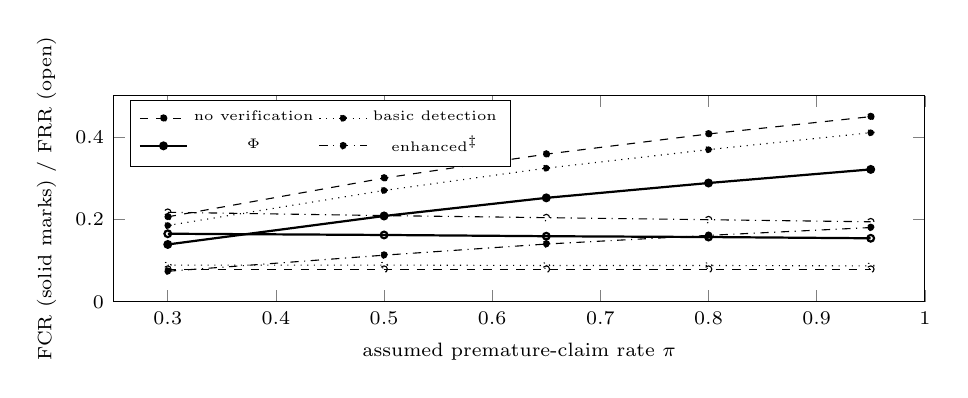
\begin{tikzpicture}
\begin{axis}[width=0.98\columnwidth, height=4.2cm, xlabel={assumed premature-claim rate $\pi$}, ylabel={FCR (solid marks) / FRR (open)},
  xmin=0.25, xmax=1.0, ymin=0, ymax=0.5, legend style={font=\tiny, at={(0.02,0.98)}, anchor=north west, legend columns=2},
  tick label style={font=\scriptsize}, label style={font=\scriptsize}]
\addplot[dashed, mark=*, mark size=1.2pt] coordinates {(0.3,0.206) (0.5,0.300) (0.65,0.358) (0.8,0.407) (0.95,0.449)};
\addlegendentry{no verification}
\addplot[dotted, mark=*, mark size=1.2pt] coordinates {(0.3,0.185) (0.5,0.270) (0.65,0.324) (0.8,0.369) (0.95,0.410)};
\addlegendentry{basic detection}
\addplot[thick, mark=*, mark size=1.2pt] coordinates {(0.3,0.139) (0.5,0.208) (0.65,0.252) (0.8,0.288) (0.95,0.321)};
\addlegendentry{$\Phi$}
\addplot[dashdotted, mark=*, mark size=1.2pt] coordinates {(0.3,0.074) (0.5,0.113) (0.65,0.140) (0.8,0.161) (0.95,0.180)};
\addlegendentry{enhanced$^{\ddagger}$}
\addplot[dashed, mark=o, mark size=1.2pt, forget plot] coordinates {(0.3,0.079) (0.5,0.079) (0.65,0.079) (0.8,0.079) (0.95,0.079)};
\addplot[dotted, mark=o, mark size=1.2pt, forget plot] coordinates {(0.3,0.089) (0.5,0.089) (0.65,0.088) (0.8,0.088) (0.95,0.087)};
\addplot[thick, mark=o, mark size=1.2pt, forget plot] coordinates {(0.3,0.165) (0.5,0.162) (0.65,0.159) (0.8,0.157) (0.95,0.154)};
\addplot[dashdotted, mark=o, mark size=1.2pt, forget plot] coordinates {(0.3,0.217) (0.5,0.209) (0.65,0.204) (0.8,0.199) (0.95,0.194)};
\end{axis}
\end{tikzpicture}
\caption{\textsc{Simulation-based (synthetic)} Study~H: mean FCR and FRR over 300 regenerated scenario sets per point as the assumed rate at which the planner claims completion of an unfinished task varies. Stricter verification lowers FCR at every rate and raises FRR; its FCR advantage grows with $\pi$. $^{\ddagger}$Not implemented.}
\label{fig:sim-sens}
\end{figure}

\begin{table}[t]
\centering
\caption{\textsc{Simulation-based (synthetic)} Study~H: robustness of the evidence-gated configuration (means over 300 regenerated sets per row, drawn from a random stream separate from the 1{,}000-set Monte Carlo of Table~\ref{tab:sim-tests}, so the unperturbed rows differ slightly from it). Without verification FCR stays at 0.36 at every continuation rate.}
\label{tab:sim-sens}
\scriptsize
\setlength{\tabcolsep}{3pt}
\begin{tabular}{@{}lccc@{}}
\toprule
Varied factor ($\Phi$) & FCR & FRR & TSR \\
\midrule
$\Phi$ detection $\times0.5$ & 0.30 & 0.14 & 0.46 \\
$\Phi$ detection $\times1.0$ & 0.25 & 0.14 & 0.47 \\
$\Phi$ detection $\times1.5$ & 0.19 & 0.13 & 0.49 \\
missing evidence 0\% & 0.23 & 0.09 & 0.52 \\
missing evidence 8\% & 0.25 & 0.14 & 0.47 \\
missing evidence 20\% & 0.29 & 0.22 & 0.39 \\
action failure rate 0.1 & 0.25 & 0.14 & 0.50 \\
action failure rate 0.25 & 0.25 & 0.14 & 0.47 \\
action failure rate 0.4 & 0.25 & 0.14 & 0.44 \\
finish after rejection 0.1 & 0.26 & 0.14 & 0.45 \\
finish after rejection 0.35 & 0.25 & 0.14 & 0.47 \\
finish after rejection 0.6 & 0.24 & 0.13 & 0.50 \\
\bottomrule
\end{tabular}
\end{table}


The advantage of verification depends on how often the planner claims completion prematurely, which is unmeasured (Fig.~\ref{fig:sim-sens}): at $\pi=0.3$ the FCR of $\Phi$ is 0.14 against 0.21 without verification, at $\pi=0.95$ 0.32 against 0.45, while FRR is constant at about 0.16 against 0.08. Halving the measured detection rate of $\Phi$ raises FCR to 0.31, close to no verification; missing evidence raises FRR because $\Phi$ fails closed on an unreadable page; more action failures lower TSR (Table~\ref{tab:sim-sens}).
